
%(BEGIN_QUESTION)
% Copyright 2012, Tony R. Kuphaldt, released under the Creative Commons Attribution License (v 1.0)
% This means you may do almost anything with this work of mine, so long as you give me proper credit

In this circuit, a type of temperature sensor called an {\it RTD} is used to generate a DC voltage signal that is read by a Programmable Logic Controller (PLC) -- a specialized type of computer built to acquire and process information from industrial sensors -- to be displayed on a graphic screen called a Human-Machine Interface (HMI):

$$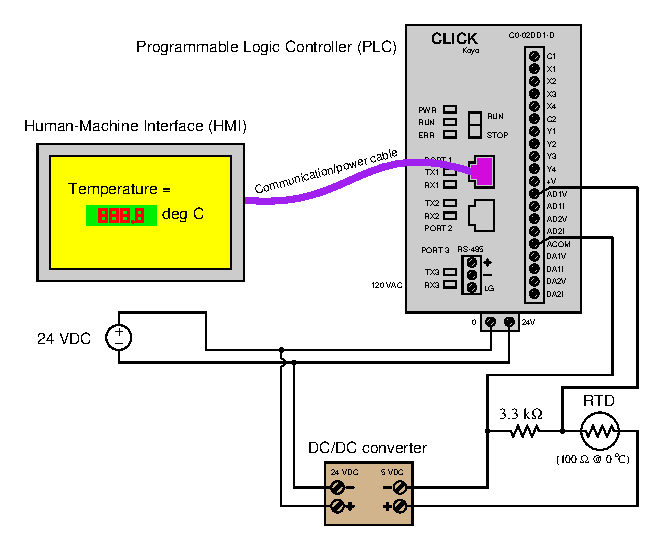
\includegraphics[width=15.5cm]{i03402x01.eps}$$

The electrical resistance of this RTD changes with temperature according to the following formula, with $R$ being the RTD's resistance in ohms and $T$ being the RTD's temperature in degrees Celsius:

$$R = 1000 (1 + 0.00385 T)$$

The analog input module of the PLC senses the voltage dropped across the 3.3 k$\Omega$ resistor, converting this signal into a digital number inside the PLC's memory directly representing volts DC.  However, no human operator looking at the HMI display will know what ``DC volts'' is supposed to mean -- he or she needs to see a display in units of {\it degrees Celsius}, not {\it volts}.

Fortunately, PLCs are {\it programmable}.  That is, you as a technician can enter a mathematical formula into the memory of the PLC to convert the voltage value into a temperature value (in degrees C).  Your task is to take the RTD formula shown above, combine it with the voltage divider formula you know from your studies of DC circuits, and write a custom formula for this application solving for $T$ in terms of $V$:

\vskip 10pt

$T$ = 

\vskip 20pt \vbox{\hrule \hbox{\strut \vrule{} {\bf Suggestions for Socratic discussion} \vrule} \hrule}

\begin{itemize}
\item{} A useful technique for double-checking your answer is to {\it work the problem backwards:} begin with your answer, working the problem in reverse to see if you arrive at the original (given) values.  Explain how to apply this technique to double-checking your answer on this particular problem.
\item{} Identify which fundamental principles of science, technology, and/or math apply to each step of your solution to this problem.  In other words, be prepared to explain the reason(s) ``why'' for every step of your solution, rather than merely describing those steps.
\item{} As the RTD temperature rises, does the voltage signal input to the PLC {\it increase} or {\it decrease}? 
\end{itemize}

\underbar{file i03402}
%(END_QUESTION)





%(BEGIN_ANSWER)

Here are the two formulae you need to begin with:
 
$$R = 1000 (1 + 0.00385 T)$$

$$V = V_{source} \left( {R \over R_{total}} \right)$$

In this particular application, we can ``flesh out'' the voltage divider formula a bit more with numerical values:

$$V = 5 \left( {3300 \over {3300 + R}} \right)$$

\vskip 10pt

After combining and manipulating these two formulae, your final formula should look something like this:

$$T = {4300 V  - 5000 \over 19.25 - 3.85 V}$$

%(END_ANSWER)





%(BEGIN_NOTES)


%INDEX% Mathematics review: manipulating and combining equations to form a new equation

%(END_NOTES)


